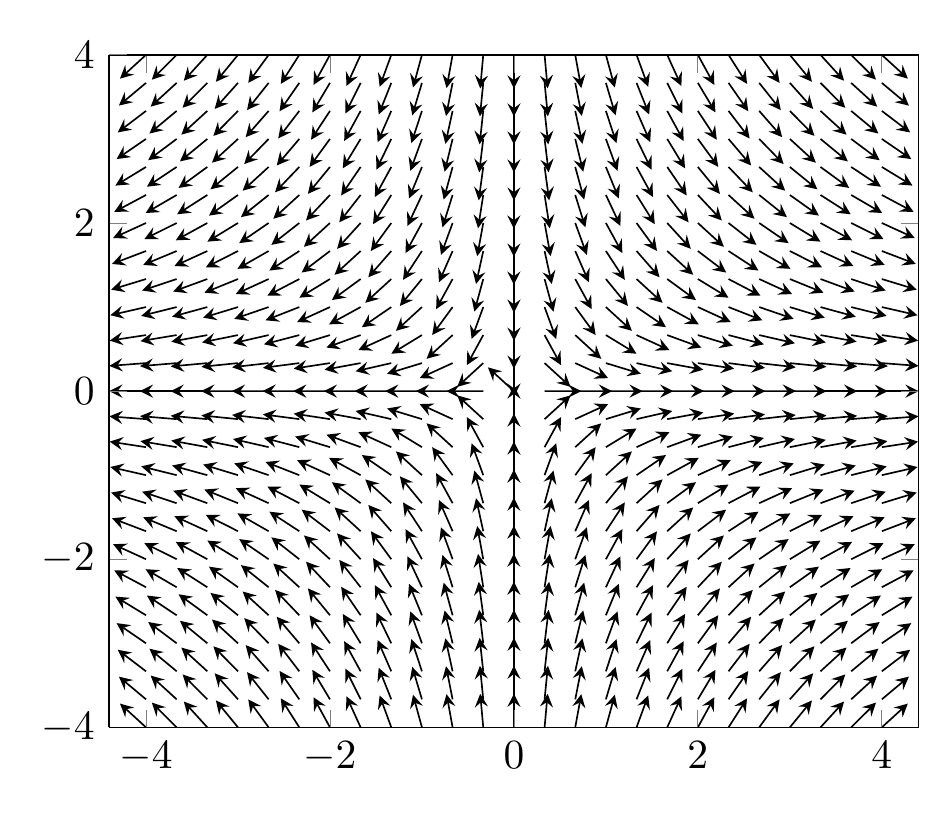
\begin{tikzpicture}[scale=1.5]
\begin{axis}[
    %Vista
    view = {0}{90},
]
    %Plotting de una funcion de variables dependientes (x,y) y dependientes (u,v) 
    \addplot3[
        %Funcion vectorial
        quiver = {
            u = {(x/(x^2+y^2))/sqrt((x/(x^2+y^2))^2+(-y/(x^2+y^2))^2)},
            v = {(-y/(x^2+y^2))/sqrt((x/(x^2+y^2))^2+(-y/(x^2+y^2))^2)},
            scale arrows = 0.4,
        },
        %Formato de flecha y restricones  
        -stealth,
        domain = -4:4,
        domain y = -4:4,
    ] {x};
\end{axis}
\end{tikzpicture}
\caption*{Representacion vectorial normalizada}
